\chapter{Event reconstruction}
\label{ch:reconstruction}

As described in Chapter~\ref{ch:lhcAndCMS}, the CMS detector
is built from complementary detector components with sensitivity
to stable particles: electrons, muons, photons, and charged
and neutral hadrons. Each can be distinguished by the likelihood of interaction
and interaction characteristics with the detector components:
all charged particles leave tracks in the tracker,
charged hadrons deposit energy in the calorimeters, photons
and electrons primarily deposite energy in the ECAL, and neutral
hadrons interact primarily with the HCAL.
The reality is more subtle than this idealized picture, illustrated
in Fig.~\ref{fig:particleFlow}, but this forms the guiding principles
in the \emph{reconstruction} of particles from their interactions in the detector.
Unstable particles are inferred by the properties of the stable particles to 
which they decay.

\begin{figure}[htbp]
  \centering
   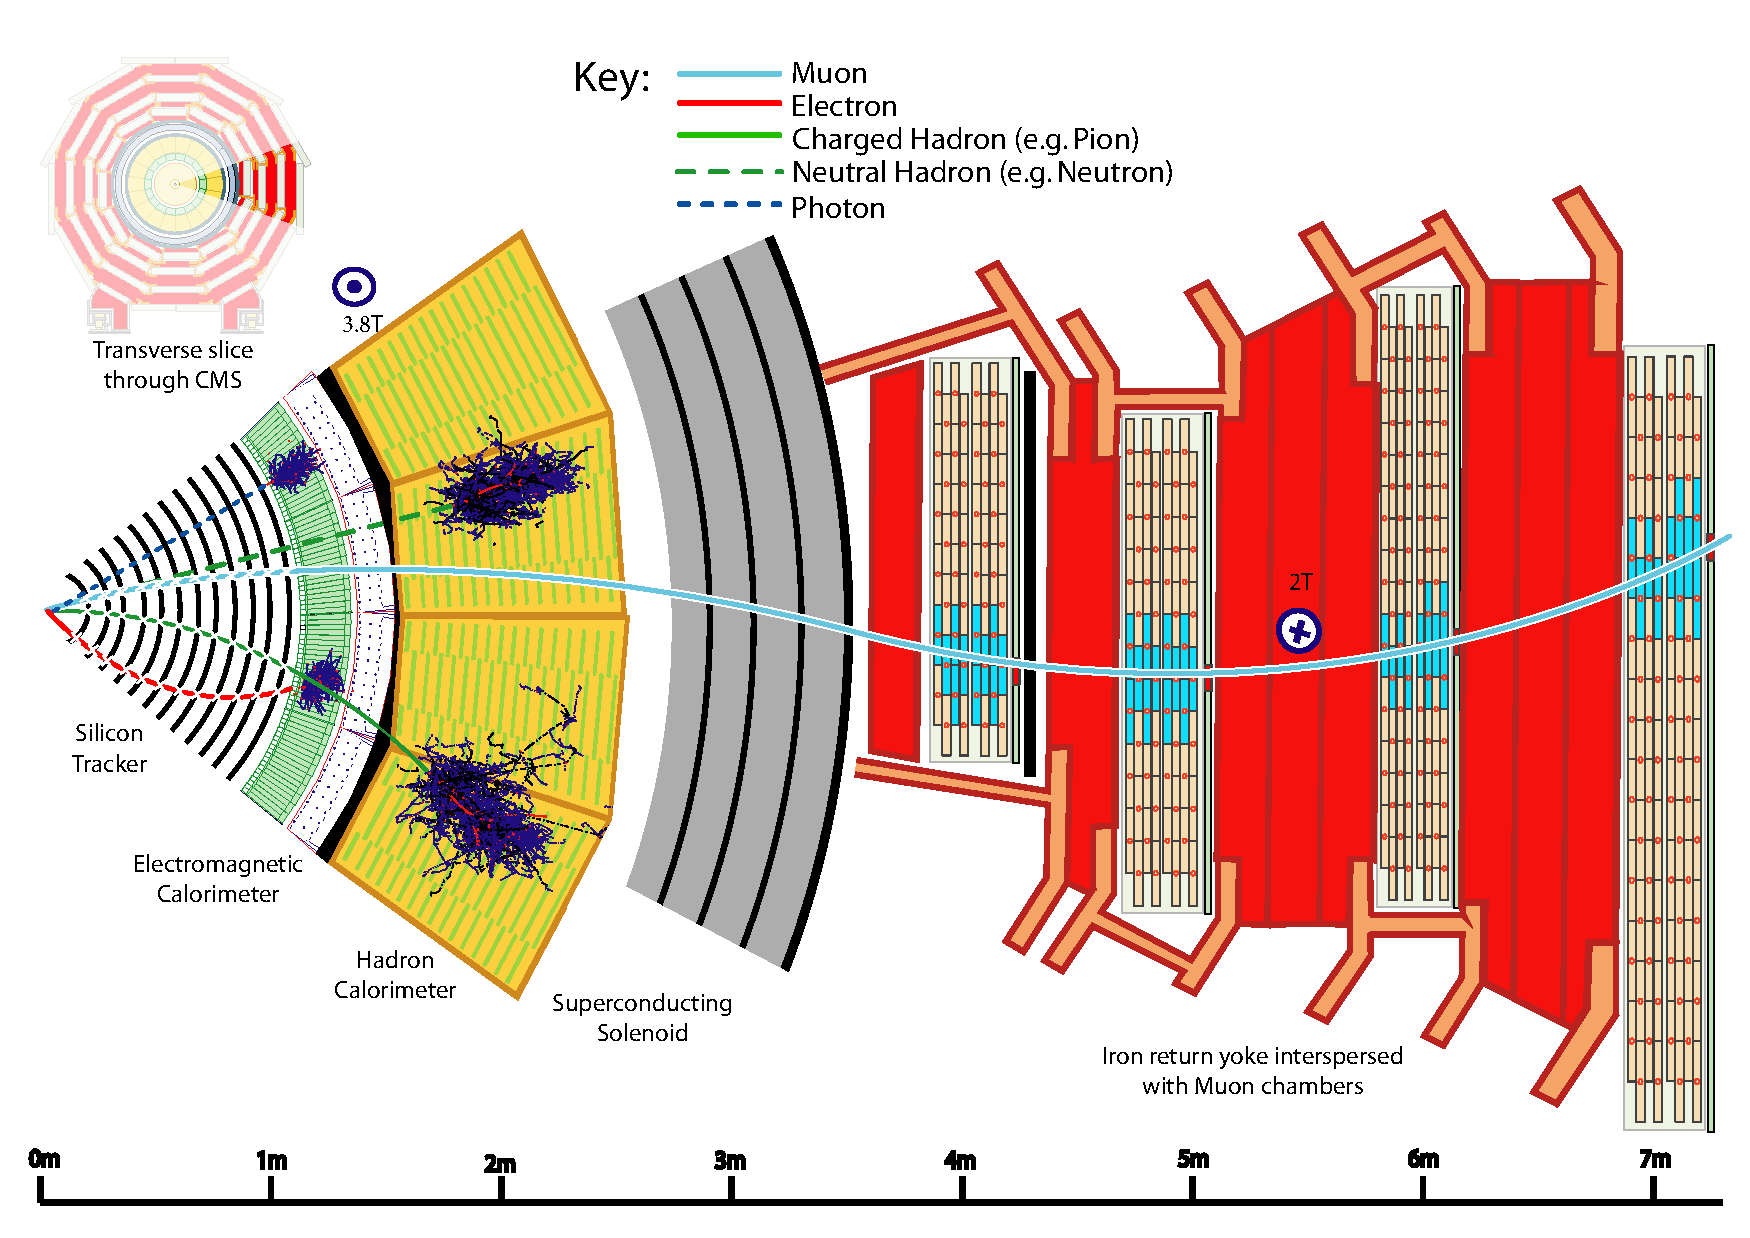
\includegraphics[width=\textwidth]{figures/Reconstruction/CMSDetectorParticleFlow.pdf}
  \caption{
    Idealized picture of particle interactions with the CMS detector subsystems.
        }
 \label{fig:particleFlow}
\end{figure}

When an event is accepted by the HLT, the raw, digitized data from each detector
subsystem is stored and simultaneously forwarded to a commercial processing farm for
further processing. Detector-specific attributes, such as signal amplitudes,
are converted to physical properties, such as energies, using calibrations
established from controlled independent measurements. System-wide patterns
are built, from which a global picture of the event and its component particles
are inferred.
The reconstruction algorithms employed by the CMS Collaboration are built from
work that began well before the LHC began taking data, 
benefiting from generations of previous experiments. The development of algorithms
is an iterative process, with continual optimizations and incremental changes
being made. The techniques described here relate to the data collection and reconstruction
used by the CMS Collaboration in 2016. Many aspects of the reconstruction
are shared by all analyses performed by the CMS Collaboration. 

A degree of ambiguity in particle identification is unavoidable. 
Reconstruction \emph{efficiency}, or a high rate of positive identification
and reconstruction of real particles, must be balanced alongside the rate of misconstruction.
For example, electrons with a poorly reconstructed track will mimic photons,
but because the track reconstruction efficiency cannot be 
accepting only very high-quality tracks will lead to a lower rate 
of indentification 
The optimal balance between efficiency and misidentification is dependent
on the characteristics of the signal and background targeted by a particular
analysis. In addition to the common reconstruction features, the identification 
criteria used in this work are also discussed.


\section{Global event description via particle flow}
The general characteristics of physics object identification outlined
above are ubiquitous amongst past, current, and future collider detector
reconstruction algorithms. Rather than applying these criteria object by
object, the CMS Collaboration exploits the 

By applying these characteristics

\subsection{Tracks and vertices}
Only energy deposits from charged particles traversing the pixel detector and
strip tracker that exceed a threshold energy (adjustable for each element)
are retained for offline storage. The position of each \emph{hit} is locally
reconstructed from clusters of adjacent pixel or strip elements based
on the relative collected charge in the cluster. 
The efficiency for hits to be reconstructed is over 99\% for active 
channels in both the pixel and strip detectors; approximately 98\%
of pixel channels and 96\% of strip channels were active during 2016 data collection.
The hit position is calculated
in local coordinates of the detector elements before being converted
into a global position with respect to the full CMS detector. The transformation
to global coordinates depends on the relative alignment of the individual tracker
elements and their alignment with respect to the other detector systems.
This is established through in situ measurements of the paths of cosmic rays
to an uncertainty neglible with respect to the intrinsic position resolution 
of the silicon detectors~\cite{Chatrchyan:2014wfa}.

The paths of charged particles through the detector are derived by 
fitting curves to the hits along a possible trajectory. 
The high combinatorics of possible track patterns that can be derived
from the large number of hits arising from high-particle-multiplicity
events is a computational challenge.
To reduce the complexity of pattern identification
while maintaining a high efficiency of reconstruction, the tracking finding
algorithm proceeds in steps, designed to first identify unambiguous
tracks before recovery those of lower quality.
Hits used to form tracks in are removed from consideration in the following
steps, reducing the complexity and chance for misassociation.

In all steps, the algorithm begins with an initial projection of the track
direction, referred to as the track \emph{seed}. The track is then formed
sequentially by extrapolating outward from the beam interaction---in the 
case of tracks seeded by the inner tracker, or inward from seeds in the muon
chambers of calorimeter clusters. Subsequent hits are located 
by predicting their location with using the
Combinatorial Track Finder (CTF) alogrithm~\cite{Chatrchyan:2014fea}, 
an adaptation of the combinatorial Kalman filter algorithm~\cite{}. 
At each step, the projected trajectory is updated to account for the additional
associated seeds, simultaneously building and fitting the particle path.
When the full trajectory through the tracker is established, the track
is refit and discarded if it fails to meet quality criteria, such as 
an excessively high $\chi^{2}$ of the fit.

The first track-forming iterations target high-quality, high-$\pt$ tracks associated
with the beam crossing region, or \emph{beam spot}, established over many
collisions by fitting the expected Gaussian beam profile to the observed
pixel tracks. These initial iterations use seeds formed from hits in each layer of 
the pixel detector, relaxed to two hits in subsequent iterations. 
Following iterations relax the requirement for the track seed to be
compatible with the beam spot, instead seeding via successive hits in the strip
tracker, increasing sensitivity
to displaced tracks from heavy-flavor hadron decays. 
Final iterations are seeded by the muon detectors using an outside-in approach.

Electrons traveling through the tracker have up to $\approx$85\% probability 
of radiating photons (known as bremsstrahlung)
due to interactions with the significant tracker material. Therefore, electron
tracks are likely to exhibit sharp kinks from sudden energy loss by bremsstrahlung.
A modified algorithm known as Gaussian sum filter (GSF)~\cite{Adam:2005bya} is thus employed to 
more accurately reconstruct electron-like tracks. In the CTF algorithm, the
Kalman filter accounts for the material interactions with a Gaussian
smearing around the expected hit location. In the GSF algorithm, 
a sum of Guassian terms, designed to reproduce the Bethe formula for electron
energy loss~\cite{doi:10.1098/rspa.1934.0140}, is used. The GSF algorithm is applied to a subset of 
tracks formed via the CTF algorithm that have few associated hits or a relatively
poor $\chi^{2}$ to obtain an improved description under the electron hypothesis.
The GSF algorithm is also used to form tracks seeded by energy clusters in the 
ECAL, described in Section~\ref{sec:ereco}.

Because the collisions analyzed for this work generally involve multiple $\pp$ interactions,
tracks originate from a variety or vertices. Vertices 
associated with a $\pp$ collision and not an interaction or decay displaced from
the collision point are identified by evaluating the common points of origin for a subset
of the track collection that are well-reconstructed (low $\chi^{2}$) and consistent with
the beam spot. No additional condition on the track $\pt$ is applied
to select this reduced track collection. The deterministic
annealing algorithm~\cite{} is used to group the tracks into their most probably set
of common vertices, before the vertex coordinates are derived by a fit to the 
associated tracks, considering their likelihood of misassignment to the vertex.

The \emph{primary vertex} is the vertex associated with the hard scattering interaction
of interest. The vertex that maximizes $\sum_{i}\pt^{2}$, where the sum considers
the tracks associated with the vertex---clustered using the anti-\kt algorithm
described in Section~\ref{sec:jreco} with radius parameter $R=0.4$---and the 
transverse momentum imbalance associated with the vertex and clustered tracks.
Studies of simulated $\WZ$ events demonstrate that this approach selects the
correct $\pp$ vertex more than 99\% of the time for signal processes considered here. 

\subsection{Muon system tracking}

\subsection{Calorimeter clusters}
Energy deposits in the calorimeter are the other crucial component of particle
identification and reconstruction in the CMS detector.

Calorimeter clusters are 
\subsection{Particle flow candidates}

\section{Physics objects}
\subsection{Muons}
Muons selected for this analysis must be identified as global muons
by the PF algorithm described previously. 
They must be within the muon detector acceptance $\abs{\eta} < 2.4$
and must have $\pt > 10\GeV$. 
Additional reconstruction
criteria are applied to reject \emph{nonprompt} muons, arising 
from hadron decays, and hadron \emph{punch through} into the muon system,
while maintaining a reconstruction efficiency greater than 96\%. 
Following the \emph{Tight} identification criteria of Ref.~\cite{},
with slight modifications,
muon candidates must satisfy:

\begin{itemize}
  \item The global muon fit must satisfy $\chi^2/\text{d.o.f.} < 10$ 
    (where d.o.f is the number of degrees of freedom in the fit) 
  \item The distance of the track vertex from the primary vertex in the $x$-$y$
    plane $d_{xy}$ must satisfy $d_{xy} < 0.2\unit{mm}$
  \item The longitudunal distance (in the $z$ plane) of the track vertex from the primary vertex 
    plane $d_{z}$ must satisfy $d_{z} < 1\unit{mm}$
  \item At least one hit in the pixel detector
  \item More than five hits in the strip tracker
  \item At least six hits in the tracker must be used in the track fit.
\end{itemize}

To reject muons from decays of hadrons in jets,
selected muons are required to be isolated from other PF objects
in the event. The relative muon isolation, the ratio of the sum of
the \pt in an $\eta$-$\phi$ region $\Delta R \def \sqrt{\eta^{2} + \phi^{2}} < 0.4$
around the muon is defined as
\begin{equation}
  I_{\mu,rel} = \frac{1}{\pt^{\mu}}\sum_{\Delta R < 0.4}\left[\pt^{h^{\pm,PV}} -  
        \max\left(\pt^{h^{0,PV}}+\pt^{\gamma} - \frac{1}{2}\pt^{h^{\pm, PU}}, 0\right)\right] \,.
\end{equation}
Here $\pt^{h^{\pm,PV}}$ and $\pt^{h^{0}}$ are, respectively, the charged and neutral hadrons
identified by the PF algorithm. The tracks of charged hadron candidates allow them to be
associated to the primary vertex, $h^{\pm,PV}$ or to pileup interactions, $h^{\pm, PU}$.
Such an assignment cannot be made reliably for neutral hadrons and photons, therefore,
all neutral hadrons and are included in the sum. To account for the expected pileup contribution,
the sum is corrected by the term $\pt^{h^{\pm}}/2$, because particle production in 
pileup interactions is expected to be dominated by charged hadron production at nearly this
ratio. A rough estimation of hadron production spit evenly beween $\pi^{+}$, $\pi^{-}$ and $\pi^{0}$ 
gives exactly this ratio, and detailed simulations confirm this expectation.

The $I_{\mu,rel}$ is used to define a baseline, or \emph{loose muon ID}, and
a signal, or \emph{tight muon ID}. Explicitly, the criteria $I_{\mu, rel} < 0.4 (0.15)$
is used for loose (tight) ID. Muons satifying the loose ID, but not the tight ID,
are to estimate the residual contamination from nonprompt muons in the event selection. 
Tight muons are used for to select signal-like events. Further description
of the approach is given in Chapter~\ref{ch:analysis}.

\subsection{Electrons}
\label{sec:ereco}
Electron selection for this analysis begins with the GSF tracks linked
to the ECAL clusters by the PF algorithm. However, unlike for muons,
selected electrons are not uniquely a subset of the PF electrons candidates.
In particular, the BDT discriminant used by the PF algorithm to
categorize electrons and photons is not considered. Instead,
binary selections are applied to specific characteristics of the
electron candidate tracks and associated clusters.

As for muons, a baseline selection is applied to electrons. Electrons
satisfying the baseline selection are used to estimate the residual
contribution from nonprompt electrons, while electrons satisfying the 
full \emph{tight ID} are selected as signal candidate events in the analysis.
The baseline selection was originally designed to mimic the electron selections applied
at the HLT level for the tightest trigger paths used in this analysis,
however, stronger conditions were applied at the HLT towards the end 
of data collection. Nonetheless, the efficiency loss is recovered by additional
trigger paths as described in Chapter~\ref{ch:analysis}.
The requirements placed on the selected \empf{loose} and \empf{tight} electron
candidates are summarized in Table~\ref{tab:elecID}. The definitions and 
purposes of the variables shown are discussed in the following.

Conditions on the GSF track and linked PF superclusters in the ECAL and HCAL
are applied to select candidates of interest. 
The track and cluster positions must be consistent, using a condition on the 
variables $\abs{\Delta\eta_{seed}}$ and $\abs{\Delta\phi_{in}}$.
The $\Delta\eta_{seed}$ is the difference between the $\eta$ direction
specified by the track seed and the $\eta$ of the PF cluster that seeds
the ECAL supercluster, and $\Delta\phi_{in}$ is the difference between
the track seed extrapolated to the supercluster and the supercluster $\phi$.
The energy threshold for electron detection ensures that the electron
mass is negligible, so the momentum measured by the track curvature and 
energy measured by the ECAL should be nearly equal. This is ensured by requiring
the variable $\pt^{track}-E^{SC}$, where $E^{SC}$ is the energy of the supercluster,
be close to zero. Electrons deposit the majority of their energy in the ECAL. 
Therefore, the ratio of the hadronic to electromagnetic energy $H/E$, measured
in terms of the PF ECAL and HCAL clusters, should be small.
To ensure a well-reconstructed track,
the baseline (loose) electron selection requires a good GSF track $\chi^2$.
For the tight identification, the track is required to have at most one
missing hit in the tracker, and the electron candidate is rejected if
any tracks consistent with a photon-to-\EE conversion are found.

The variable $\sigma_{i\eta i\eta}$ is used to assess the shape of the shower
in the $\eta$. It is defined as
\begin{equation}
  \sigma_{i\eta i\eta} = \sqrt{\sum_{i\in 5\times5}\frac{ w_{i}(i\eta_{i} - \bar{i\eta})}{w_i^2}}\,,
\end{equation}
where the sum is over the $5\times5$ block of ECAL crystals centered around the
cluster seed, and the weights $w_i$ are defined as
\begin{equation}
  w_i = \max\left(0, 4.7+\ln{\frac{E_i}{E_{5\times5}}}\right)\,.
\end{equation}
The variable $i\eta_i$ is the $\eta$ of each crystal in the sum,
expressed in integer units numbering the crystals, a choice that allows the variable
gaps between crystals to be ignored. In the endcaps, the arrangement of crystals
is in the $x$-$y$ plane, and $i\eta\def \sqrt{ix^2+iy^2}$ with crystal integer 
numbering $ix$. The $\bar{i\eta}$ is the $i\eta$ of the $5\times5$ cluster,
$E_i$ is the energy of the $i$th crystal, and $E_{5\times5}$ ise the energy 
sum of the $5\times5$ cluster.

As for muons, selected electrons must be isolated from other event activity.
The definition of the isolation depends on the physics objects considered in the sum,
and the approach to pileup substraction.
For the loose electrons selection, the isolation is defined in terms of the tracks,
and the PF energy clusters in the ECAL and HCAL contained in a cone defined by 
$\Delta R < 0.3$ around the electron. The sum of ECAL and HCAL cluster energies 
are corrected by estimated the pileup energy contribution per event using the 
\emph{effective area} technique proposed for jets in Ref. 
The isolation is defined as
\begin{equation}
  I_{\mu,rel} = \frac{1}{\pt^{\mu}}\sum_{\Delta R < 0.3}\left[\pt^{h^{\pm,PV}} -  
        \max\left(\pt^{h^{0,PV}}+\pt^{\gamma} - \frac{1}{2}\pt^{h^{\pm, PU}}, 0\right)\right] \,.
\end{equation}



Because the ECAL measurement is more complex, and because the pileup contributions
are larger in the ECAL than in the muon system, a more complex method of pileup subtracking is applied.




\begin{table}[htbp]
    \centering
    \caption[]{
            }
    \begin{tabular}{lcccc} 
                        & \multicolumn{2}{c}{Baseline ID} & \multicolumn{2}{c}{Tight ID}  \\
      Variable                & ECAL barrel & ECAL endcap & ECAL barrel & ECAL endcap        \\
    \hline
      $\abs{\Delta\eta_{seed}}$ & 0.004     & ---         & 0.00308     & 0.0605 \\
      $\abs{\Delta\phi_{in}}$   & 0.020     & ---         & 0.0816      & 0.0394 \\
      $\abs{E_{SC}^{-1} - p_{track}^{-1}}$  & \multicolumn{2}{c}{0.013} & 0.0129 & 0.0129 \\
      $\sigma_{i\eta i\eta}$  & 0.011       & 0.031       & 0.00998     & 0.0298 \\
      $H/E$                   & 0.060     & 0.065       & 0.0414      & 0.0641 \\
      $I^{ECAL}$        & 0.160     & 0.120       & \multicolumn{2}{c}{1} \\
      $I^{HCAL}$        & \multicolumn{2}{c}{0.120} & \multicolumn{2}{c}{1} \\
      $I^{track}$       & \multicolumn{2}{c}{0.08} & \multicolumn{2}{c}{1} \\
      $I_{e,rel}^{PF,corr}$     & \multicolumn{2}{c}{---} & 0.0588      & 0.0571 \\
      GSF track $\chi^{2}/\text{d.o.f.}$  & ---                     & 3.0         & \multicolumn{2}{c}{---} \\
      Max missing tracker hits  & \multicolumn{2}{c}{---} & \multicolumn{2}{c}{1} \\
    \hline 
     \end{tabular}
    \label{tab:elecID}
\end{table}
  \subsection{Charged and neutral hadrons}
  \subsection{Jets}
  \subsection{Identification b-jets}
  \subsection{Missing transverse momentum}

